\section{FECG analysis}
FECG is the fetal ECG superimposed over the maternal ECG. ECG measurement is a cocktail party where on source is measured over different electrodes.

Application of the ICA on the FECG data tends to decrease the interference coming from other sources at the region where the electrodes of the interest is placed. However in this "cocktail" effect the outcome is not with benefits in all the cases. Hereby in figure \ref{FECG1} and \ref{FECG1} the signals before and after applying BSS-ICA. The original signal tends to contain a lot of interference where fetal signal with small amplitude is also incorporated into the underlying signal. This peaks could potentially disappear after the ICA since their correlation with noise is much higher compare to the correlation with the real high amplitude signal. Consequently after ICA these peaks mainly disappear.  Nevertheless these weak fetal signal could potentially be important information for the analysis and risk assessment of the fetal. 

BSS over this dataset is quite efficient where a clear QRS signal is feasible together with the P and T waves which are visually disclosed from the figure \ref{FECG1}. The artefat and the crosstalk that presented in the original signal are suppressed and the quality of the final signal is sufficiently good.

Even though ICA is a very powerful tool in processing ECG signals it is still not a suitable framework for fetal ECG processing. Further processing of the FECG signal could be of great importance using wavelet and filtering in order to extract more hidden information. 

\begin{figure}[!htbp]
\minipage{0.5\textwidth}%
\centering
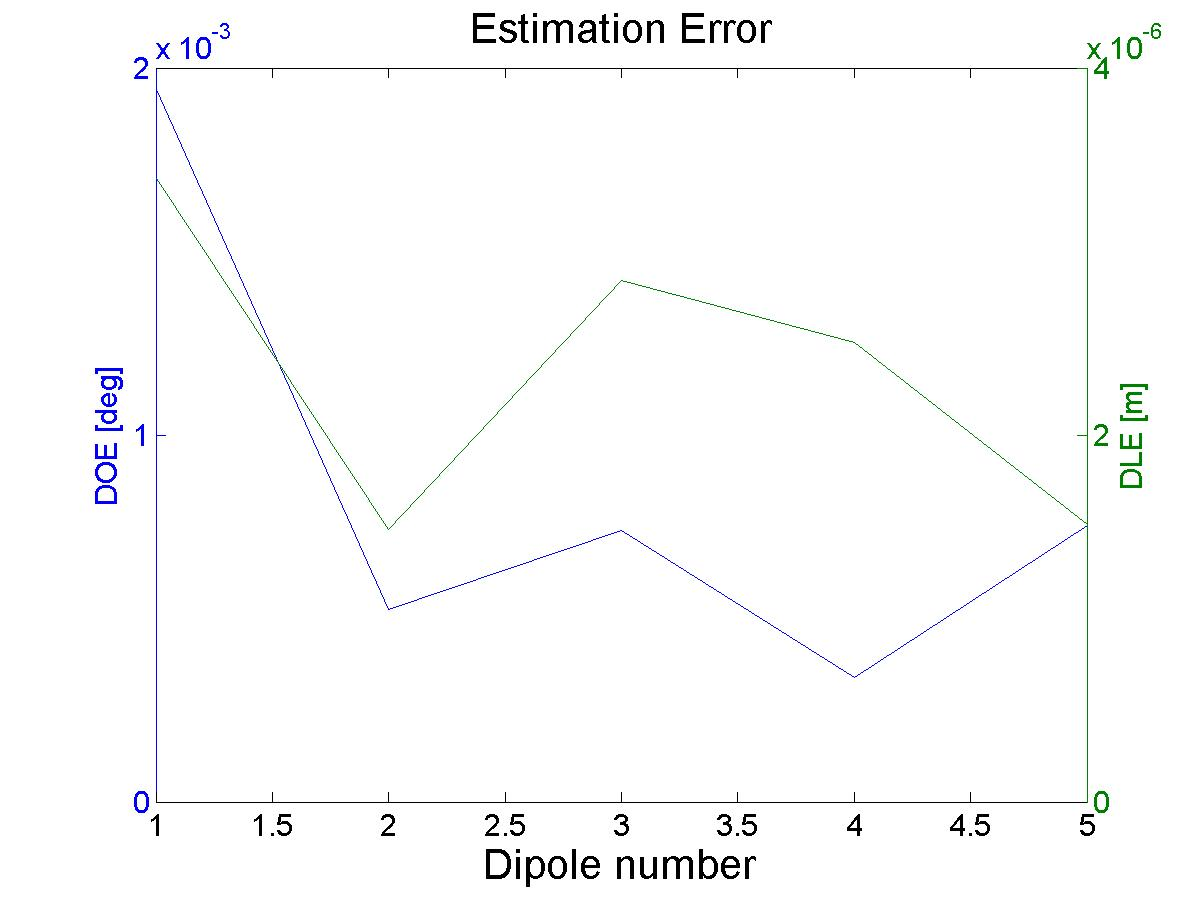
\includegraphics[width=1\linewidth]{100.jpg}
\subcaption{FECG before BSS}\label{FECG2}
\endminipage\hfill
\minipage{0.5\textwidth}%
\centering
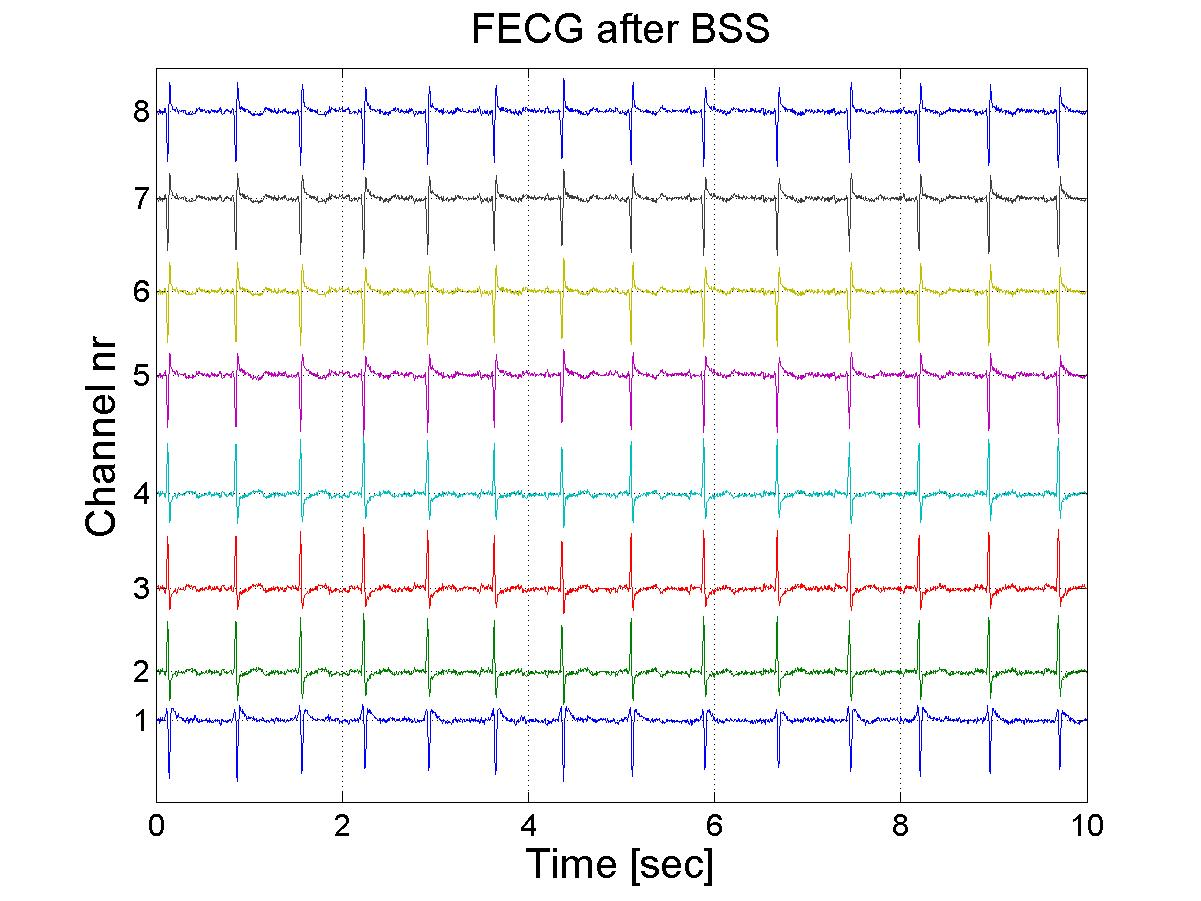
\includegraphics[width=1\linewidth]{101.jpg}
\subcaption{FECG after BSS}\label{FECG1}
\endminipage\hfill
\caption{BSS over FECG.}
\end{figure}